\documentclass[12pt,a4paper]{report}
% Layout shared by the coursework reports in this repository.
\usepackage{fontspec}
\IfFontExistsTF{DejaVu Sans Mono}{\setmonofont[Scale=0.84]{DejaVu Sans Mono}}{}
\usepackage[vietnamese]{babel}
\usepackage[a4paper,margin=1in]{geometry}
\usepackage{amsmath,amssymb,mathtools,bm}
\usepackage{booktabs,tabularx,array,longtable}
\usepackage{graphicx,float}
\usepackage{enumitem}
\usepackage{fancyhdr,setspace,titlesec,caption,microtype,needspace,etoolbox}
\usepackage[hidelinks]{hyperref}

\setstretch{1.15}
\setlength{\parskip}{0.45em}
\setlength{\parindent}{0pt}
\setlength{\headheight}{16pt}
\setcounter{tocdepth}{2}
\setcounter{secnumdepth}{3}
\emergencystretch=2em

\captionsetup{font=small,labelfont=bf}
\numberwithin{equation}{chapter}

\titleformat{\chapter}[display]
  {\normalfont\bfseries}
  {\filleft\Large\chaptertitlename\ \thechapter}
  {0.35em}
  {\filright\huge}
  [\vspace{0.4em}\titlerule]
\titlespacing*{\chapter}{0pt}{-10pt}{22pt}
\titleformat{\section}{\Large\bfseries}{\thesection}{0.6em}{}
\titleformat{\subsection}{\large\bfseries}{\thesubsection}{0.6em}{}
\titleformat{\subsubsection}{\normalsize\bfseries}{\thesubsubsection}{0.6em}{}

\preto\section{\Needspace{5\baselineskip}}{}
\preto\subsection{\Needspace{4\baselineskip}}{}
\preto\subsubsection{\Needspace{3\baselineskip}}{}

\newcommand{\CourseReportHeader}[1]{%
  \pagestyle{fancy}%
  \fancyhf{}%
  \fancyhead[L]{\small\nouppercase{\leftmark}}%
  \fancyhead[R]{\small #1}%
  \fancyfoot[C]{\thepage}%
  \fancypagestyle{plain}{%
    \fancyhf{}%
    \fancyhead[L]{\small\nouppercase{\leftmark}}%
    \fancyhead[R]{\small #1}%
    \fancyfoot[C]{\thepage}%
  }%
}

\newcommand{\R}{\mathbb{R}}
\newcommand{\norm}[1]{\left\lVert #1 \right\rVert}
\newcommand{\code}[1]{\texttt{\detokenize{#1}}}

% Arguments: logo, report type, course, title, author label, metadata rows, date.
\newcommand{\CourseCover}[7]{%
  \hypersetup{pageanchor=false}%
  \begin{titlepage}
    \centering
    \vspace*{0.5cm}
    {\normalsize\bfseries ĐẠI HỌC QUỐC GIA THÀNH PHỐ HỒ CHÍ MINH\par}
    {\normalsize\bfseries TRƯỜNG ĐẠI HỌC BÁCH KHOA\par}
    {\normalsize\bfseries KHOA KHOA HỌC VÀ KỸ THUẬT MÁY TÍNH\par}
    \vspace{0.6cm}
    \includegraphics[width=0.2\textwidth]{#1}\par
    \vspace{0.7cm}
    {\large\bfseries #2\par}
    \vspace{0.35cm}
    {\normalsize\textbf{#3}\par}
    {\small Học kỳ 261 · Năm học 2026–2027\par}
    \vspace{0.45cm}
    {\LARGE\bfseries #4\par}
    \vspace{0.6cm}
    {\normalsize\bfseries #5\par}
    \vspace{0.35cm}
    {\small\begin{tabular}{@{}ll@{}}#6\end{tabular}\par}
    \vfill
    {\small\bfseries Thành phố Hồ Chí Minh, #7\par}
  \end{titlepage}
  \pagenumbering{roman}%
  \hypersetup{pageanchor=true}%
}

\newcommand{\CourseFrontChapter}[1]{%
  \chapter*{#1}%
  \addcontentsline{toc}{chapter}{#1}%
  \markboth{#1}{#1}%
}

\newcommand{\CourseAbstract}[1]{%
  \CourseFrontChapter{Tóm tắt}%
  #1\par
}

\newcommand{\CourseOverview}[1]{%
  \CourseFrontChapter{Tổng quan báo cáo}%
  \begingroup
  \renewcommand{\arraystretch}{1.3}%
  \begin{tabularx}{\textwidth}{@{}>{\bfseries\raggedright\arraybackslash}p{3.3cm}>{\raggedright\arraybackslash}X@{}}
    #1
  \end{tabularx}
  \endgroup
}

% Omit the figure list for a report containing only tables.
\newcommand{\CourseContents}[1][\listoffigures]{%
  \tableofcontents
  #1%
  \listoftables
  \clearpage
  \pagenumbering{arabic}%
}

\CourseReportHeader{CO5177 · Image}
\newcommand{\resultfigure}[3]{\begin{figure}[htbp]\centering\includegraphics[width=#3\textwidth]{notebook-evidence/figures/#1.png}\caption{#2}\end{figure}}
\hypersetup{pdftitle={CO5177 - Bao cao Image},pdfauthor={Huynh Thanh Dat; Luong Minh Duy}}

\begin{document}
\CourseCover{assets/hcmut-logo.png}
  {BÁO CÁO IMAGE}
  {CO5177 · Nền tảng lập trình cho phân tích và trực quan dữ liệu}
  {Phân loại CIFAR-100 bằng ResNet18 và Swin-T}
  {Nhóm CTG}
  {Huỳnh Thành Đạt & 2570161 · 50\%\\
   Lương Minh Duy & 2570083 · 50\%\\[0.5em]
   Giảng viên & Lê Thành Sách}
  {tháng 11 năm 2026}

\CourseAbstract{
Thực nghiệm so sánh ba mức fine-tuning của ResNet18 và Swin-T pretrained ImageNet trên CIFAR-100. Trước khi huấn luyện, các ảnh trùng pixel chính xác được loại giữa các tập theo một chính sách ưu tiên cố định, tạo tập train/validation/test gồm 44.976/5.000/9.998 ảnh. Sáu cấu hình pretrained được huấn luyện 20 epoch với ba seed. Swin-T ở chế độ full fine-tuning đạt accuracy test $86{,}81\pm0{,}02$\%, cao hơn ResNet18 cùng chế độ $7{,}66\pm0{,}41$ điểm phần trăm khi so sánh theo cặp seed. Thời gian train trung bình của Swin-T full gấp 2,63 lần và bộ nhớ cấp phát cực đại gấp 4,72 lần ResNet18 full.
}

\CourseOverview{
Dữ liệu & CIFAR-100, 100 lớp; ảnh gốc $32\times32$, đầu vào $96\times96$.\\
Split & 44.976 train, 5.000 validation, 9.998 test sau khi loại ảnh trùng chính xác.\\
Mô hình & ResNet18 và Swin-T pretrained ImageNet; head-only, partial và full fine-tuning.\\
Kết quả chính & Swin-T full đạt $86{,}81\pm0{,}02$\% accuracy và macro-F1 $0{,}8681\pm0{,}0001$.\\
Đánh đổi & Accuracy cao hơn đi kèm 2,63 lần thời gian và 4,72 lần bộ nhớ so với ResNet18 full.
}

\CourseContents

\chapter{Bài toán và dữ liệu}
\section{Mục tiêu}
Thực nghiệm khảo sát ảnh hưởng của mức độ cập nhật backbone khi phân loại CIFAR-100. Hai kiến trúc ResNet18 và Swin-T sử dụng trọng số ImageNet-1K phiên bản V1. Mỗi kiến trúc được đánh giá ở ba chế độ pretrained: chỉ học lớp phân loại (head-only), fine-tuning một phần backbone (partial) và fine-tuning toàn bộ (full). Tất cả sáu cấu hình được chạy với seed 42, 43 và 44.

Mục tiêu là so sánh chất lượng dự đoán và chi phí thực thi trong cùng ngân sách 20 epoch. Kết luận giới hạn ở hai kiến trúc và bộ trọng số pretrained được chọn.

\section{Dữ liệu và kích thước ảnh}
CIFAR-100 do Đại học Toronto công bố, gồm 60.000 ảnh màu thuộc 100 lớp chi tiết (fine label), được nhóm thành 20 lớp tổng quát (coarse label): 50.000 ảnh train chính thức và 10.000 ảnh test chính thức \cite{cifar}. Bản Python được phân phối dưới dạng tệp pickle \code{train}, \code{test} và \code{meta}; hai tệp dữ liệu chứa các mảng pixel cùng nhãn fine/coarse, còn \code{meta} chứa tên lớp. Thực nghiệm phân loại theo 100 fine label.

Ảnh gốc có kích thước $32\times32$; toàn bộ dữ liệu nguồn được đưa vào bước chia và loại trùng. Đề bài khuyến nghị, không bắt buộc, cạnh ngắn ít nhất 128 px \cite{assignment}. Thực nghiệm dùng đầu vào $96\times96$ cho cả hai kiến trúc và mọi mức fine-tuning để kiểm soát điều kiện so sánh. Đây là lựa chọn cân bằng giữa kích thước đầu vào và chi phí tính toán: ảnh được phóng lớn ba lần theo mỗi chiều, nhưng số điểm ảnh đầu vào vẫn thấp hơn khi dùng 128 px. Nội suy song tuyến tính không bổ sung chi tiết ngoài ảnh gốc. Vì chưa đối chiếu trực tiếp 96 px với 128 px, kết quả không cho biết mức ảnh hưởng của lựa chọn kích thước này đến accuracy.

Từ 50.000 ảnh train, phép chia phân tầng với seed 2026 ban đầu tạo 45.000 ảnh train và 5.000 ảnh validation. Trước khi train, các ảnh có nội dung pixel RGB giống hệt nhau được nhóm lại trong cả ba tập. Mỗi nhóm giữ một ảnh theo thứ tự ưu tiên test, validation, rồi train. Chính sách này loại 24 ảnh khỏi train và 2 khỏi test; validation không đổi. Tập cuối gồm 44.976/5.000/9.998 ảnh. Đối chiếu sau lọc xác nhận không còn nội dung RGB trùng chính xác giữa các tập. Phép kiểm tra chưa xét ảnh gần trùng hoặc mức độ tương đồng thị giác.

\begin{figure}[htbp]\centering
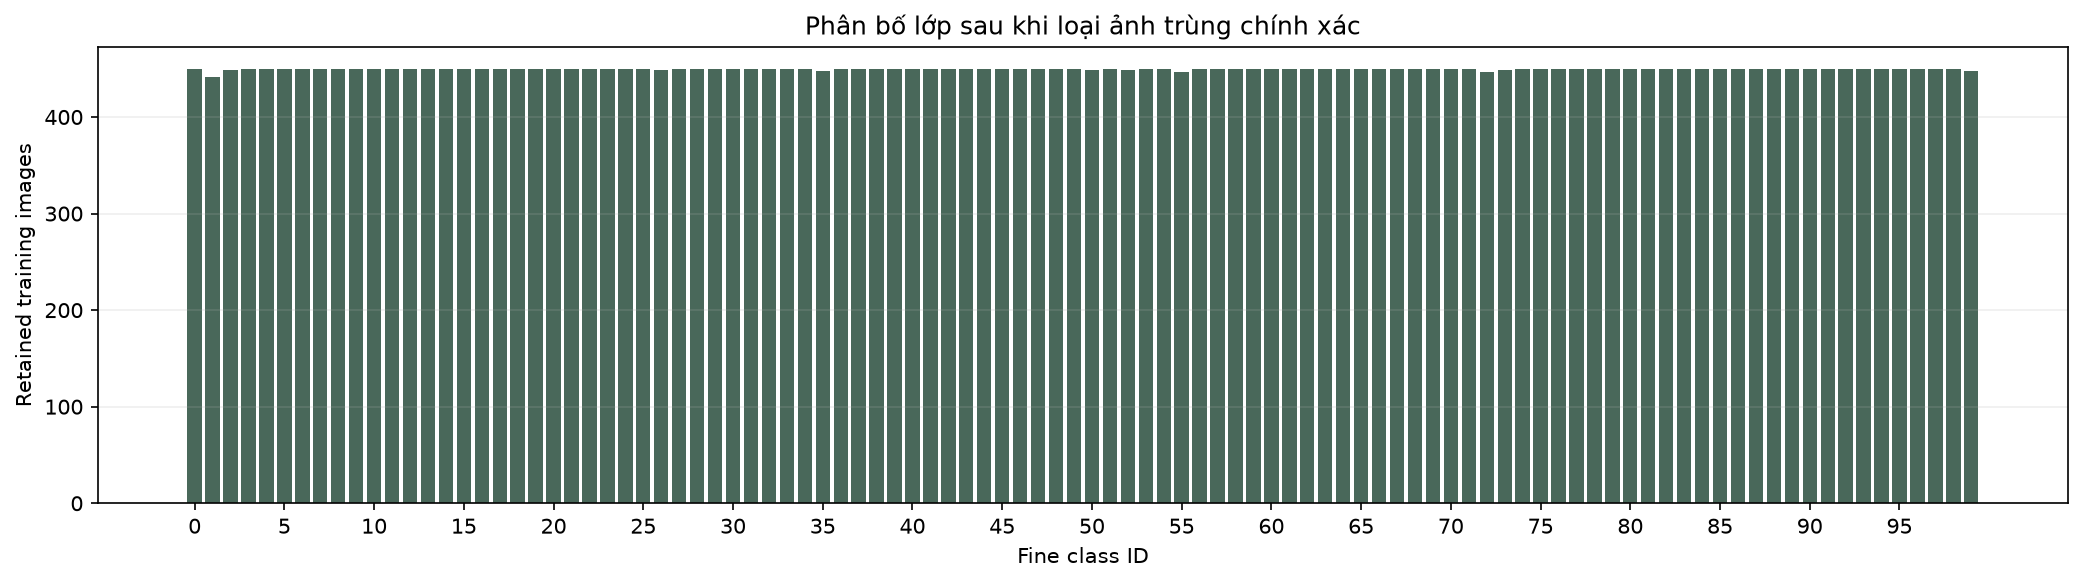
\includegraphics[width=.91\textwidth]{notebook-evidence/figures/class_distribution.png}
\caption{Số ảnh theo lớp sau khi loại nội dung trùng chính xác. Các lớp vẫn có quy mô gần tương đương; tiêu chí loại trùng là nội dung pixel RGB giống hệt nhau.}
\end{figure}

\begin{figure}[htbp]\centering
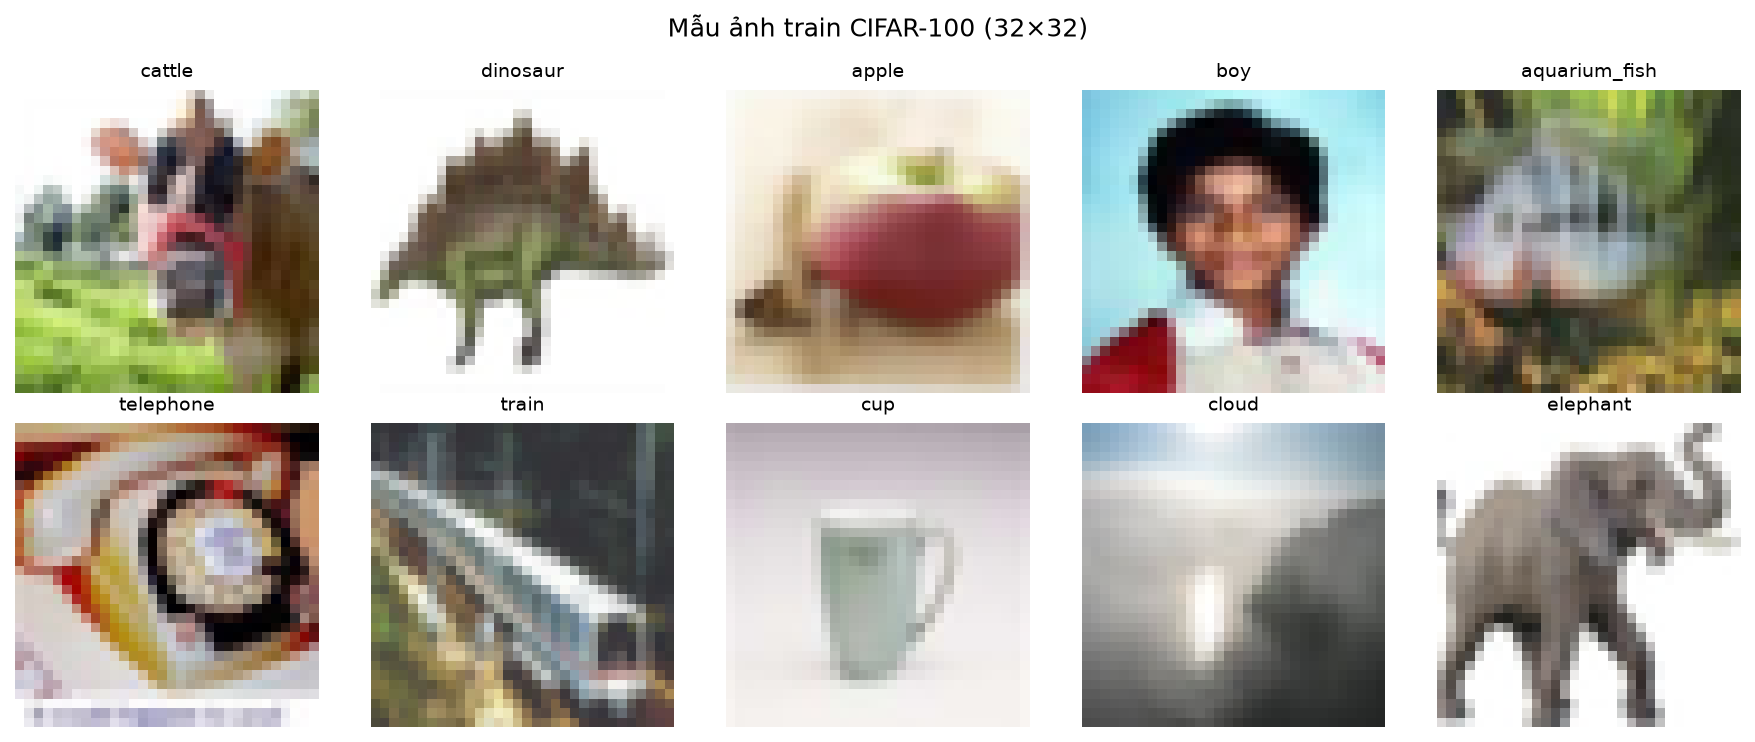
\includegraphics[width=.78\textwidth]{notebook-evidence/figures/training_examples.png}
\caption{Mẫu ảnh CIFAR-100 trong tập train sau khử trùng lặp. Ảnh nguồn $32\times32$ có một số lớp khó phân biệt khi chỉ quan sát hình dạng và kết cấu tổng thể.}
\end{figure}

\section{Tiền xử lý}
Ảnh trong tập train được áp dụng padding 4 pixel, random crop về $32\times32$, random horizontal flip với xác suất 0,5 rồi resize lên $96\times96$ bằng nội suy song tuyến tính. Random crop thay đổi vị trí vật thể trong khung ảnh; random horizontal flip bổ sung các biến thể đối xứng ngang. Ảnh trong tập validation và test chỉ được resize về kích thước cố định. Sau khi chuyển giá trị pixel về $[0,1]$, cả ba tập đều được áp dụng normalization theo từng kênh màu: $x_c^{\prime}=(x_c-\mu_c)/\sigma_c$, với $\mu=(0{,}485;0{,}456;0{,}406)$ và $\sigma=(0{,}229;0{,}224;0{,}225)$. Cách xử lý này đưa đầu vào về thang giá trị tương ứng với trọng số pretrained ImageNet. Augmentation chỉ áp dụng cho train; validation dùng chọn checkpoint và test chỉ được đánh giá sau khi giao thức đã cố định.

\chapter{Mô hình và thiết lập thực nghiệm}
\section{Đặc trưng ảnh và cơ chế phân loại}
ResNet18 trích xuất đặc trưng bằng các lớp convolution và các khối residual \cite{resnet}. Khi kích thước phù hợp, một khối có dạng $h_{l+1}=\operatorname{ReLU}(F_l(h_l)+h_l)$: nhánh convolution học phần biến đổi $F_l$, còn nhánh tắt giữ đường truyền trực tiếp cho đặc trưng và gradient. Sau các khối này, global average pooling tổng hợp đặc trưng không gian trước lớp phân loại.

Swin-T chia ảnh thành các patch và tính self-attention trong từng cửa sổ, đồng thời luân phiên dịch cửa sổ để trao đổi thông tin giữa các vùng lân cận \cite{swin}. Với một attention head, phép tính có dạng
\[
\operatorname{Attention}(Q,K,V)=\operatorname{softmax}\!\left(\frac{QK^{\mathsf T}}{\sqrt{d}}+B\right)V,
\]
trong đó $Q,K,V$ là các phép chiếu của đặc trưng patch, $d$ là số chiều của key và $B$ biểu diễn độ lệch vị trí tương đối. Qua các stage, patch merging giảm độ phân giải không gian và tăng số kênh đặc trưng. Hai kiến trúc vì vậy khác nhau cả về cách kết hợp thông tin không gian lẫn cấu trúc backbone; phép so sánh hiện tại không tách riêng tác động của từng khác biệt.

Với đặc trưng ảnh $h_\theta(x)$, lớp phân loại mới tạo 100 logit $z=Wh_\theta(x)+b$. Xác suất lớp $c$ là $p_c=\exp(z_c)/\sum_{k=1}^{100}\exp(z_k)$ và nhãn dự đoán là $\arg\max_c p_c$. Cả hai mô hình thay head ImageNet bằng lớp Linear có 100 đầu ra để phù hợp với nhãn CIFAR-100.

\section{Các mức fine-tuning}
ResNet18 sử dụng backbone torchvision pretrained \cite{resnet,torchvision}. Head-only chỉ cập nhật lớp Linear 100 chiều; partial cập nhật layer4 và head; full cập nhật toàn bộ mô hình. Swin-T cũng dùng pretrained ImageNet \cite{swin,torchvision}: head-only chỉ cập nhật head, partial cập nhật stage cuối, normalization cuối và head, còn full cập nhật toàn bộ backbone.

\begin{table}[htbp]\centering
\begin{tabularx}{\textwidth}{@{}l l X@{}}
\toprule
Chế độ & Khởi tạo & Tham số được cập nhật\\\midrule
Head-only & ImageNet pretrained & Lớp phân loại 100 chiều\\
Partial & ImageNet pretrained & Khối cuối và lớp phân loại; Swin-T thêm normalization cuối\\
Full & ImageNet pretrained & Toàn bộ mô hình\\
\bottomrule
\end{tabularx}
\caption{Phạm vi tham số được cập nhật ở ba chế độ fine-tuning. Cả hai kiến trúc dùng cùng cách chia dữ liệu, tiền xử lý và seed.}
\end{table}

Head-only kiểm tra khả năng phân loại từ đặc trưng pretrained khi chỉ học ranh giới quyết định mới. Partial cho phép điều chỉnh đặc trưng ở khối cuối, còn full cho phép thích nghi ở mọi tầng. Các phần đóng băng được giữ ở chế độ đánh giá để không cập nhật thống kê BatchNorm hoặc kích hoạt stochastic depth trong những phần đó. Nhờ vậy, head-only thực sự giữ cố định backbone trong quá trình train.

\section{Huấn luyện và đánh giá}
Mỗi lượt chạy 20 epoch, batch size 128, AdamW với weight decay $10^{-4}$ và cosine learning-rate schedule. Learning rate ban đầu là $10^{-3}$ cho head-only và $10^{-4}$ cho partial/full. Loss là cross-entropy không label smoothing; gradient norm được clip ở 1. Autocast BF16 dùng trên GPU hỗ trợ BF16 native; tham số và trạng thái optimizer ở FP32, TF32 tắt. Checkpoint được chọn theo validation accuracy cao nhất; khi hòa chọn validation cross-entropy thấp hơn.

Với batch gồm $m$ ảnh và nhãn đúng $y_i$, hàm mất mát được tối thiểu hóa là
\[
\mathcal{L}_{\mathrm{CE}}=-\frac{1}{m}\sum_{i=1}^{m}\log p_{i,y_i}.
\]
Cross-entropy phạt dự đoán gán xác suất thấp cho nhãn đúng, trong khi accuracy chỉ xét nhãn có xác suất lớn nhất. Vì thế, hai đại lượng có thể biến đổi khác nhau khi mô hình trở nên tự tin hơn. Learning rate nhỏ hơn ở partial/full nhằm hạn chế thay đổi quá mạnh các tham số pretrained. Tuy nhiên, vì head-only dùng learning rate khác, chênh lệch với chế độ này phản ánh toàn bộ thiết lập fine-tuning, chưa phải tác động riêng của số tầng được cập nhật.

Accuracy là tỷ lệ ảnh được phân loại đúng. Macro-F1 tính $F1_c=2TP_c/(2TP_c+FP_c+FN_c)$ cho từng lớp rồi lấy trung bình $\frac{1}{100}\sum_c F1_c$, nên mỗi lớp có trọng số như nhau. Dù các lớp CIFAR-100 gần cân bằng, báo cáo đồng thời hai chỉ số giúp kiểm tra mức độ nhất quán giữa chất lượng dự đoán chung và chất lượng trung bình theo lớp.

Kết quả được đo trên RTX 5090 với bốn worker nạp dữ liệu, PyTorch 2.10.0, torchvision 0.25.0, CUDA 13.0, NumPy 2.5.4, Matplotlib 3.11.2 và Pillow 12.3.0. Thời gian train gồm nạp dữ liệu, augmentation và lượt huấn luyện, có đồng bộ CUDA; không gồm validation, khởi tạo mô hình, ghi checkpoint hoặc xuất báo cáo. Peak memory là bộ nhớ GPU cấp phát cực đại trong train và validation của mỗi lượt. Accuracy và macro-F1 được tính trên toàn bộ lớp; các giá trị tổng hợp là trung bình và độ lệch chuẩn mẫu qua ba seed.

\chapter{Kết quả và thảo luận}
% Kết quả tổng hợp từ 18 lượt train; độ lệch chuẩn là SD mẫu.
\section{Kết quả trên tập test}

Bảng~\ref{tab:new-image-results} tổng hợp accuracy và macro-F1 trên 9.998 ảnh trong tập test sau khi loại trùng pixel chính xác. Ở cả hai kiến trúc, chế độ partial vượt head-only; full tiếp tục cải thiện kết quả. ResNet18 full đạt $79{,}16\pm0{,}39$\%, còn Swin-T full đạt $86{,}81\pm0{,}02$\%.

\begin{table}[htbp]\centering\small
\setlength{\tabcolsep}{5pt}
\begin{tabular}{lrr}
\toprule
Cấu hình & Accuracy test (\%) & Macro-F1\\\midrule
ResNet18 head-only & $60{,}91\pm0{,}14$ & $0{,}6077\pm0{,}0012$\\
ResNet18 partial & $73{,}84\pm0{,}23$ & $0{,}7382\pm0{,}0018$\\
ResNet18 full & $79{,}16\pm0{,}39$ & $0{,}7915\pm0{,}0038$\\
Swin-T head-only & $71{,}69\pm0{,}07$ & $0{,}7156\pm0{,}0008$\\
Swin-T partial & $78{,}44\pm0{,}16$ & $0{,}7837\pm0{,}0015$\\
Swin-T full & $86{,}81\pm0{,}02$ & $0{,}8681\pm0{,}0001$\\
\bottomrule
\end{tabular}
\caption{Full cho accuracy cao nhất trong từng kiến trúc. Swin-T full đạt 86,81\% so với 79,16\% của ResNet18 full, cao hơn 7,66 điểm phần trăm theo so sánh ghép cặp cùng seed. Accuracy và macro-F1 được trình bày dưới dạng trung bình $\pm$ SD mẫu qua seed 42, 43 và 44.}
\label{tab:new-image-results}
\end{table}

Mức tăng khi mở thêm backbone khác nhau giữa hai kiến trúc. Với ResNet18, phần cải thiện lớn hơn xuất hiện từ head-only sang partial; với Swin-T, bước từ partial sang full đem lại mức tăng lớn hơn bước từ head-only sang partial. Như vậy, cập nhật riêng khối cuối chưa khai thác hết chất lượng đạt được của Swin-T trong ngân sách này. Tuy nhiên, các kết quả không xác định được tầng nào tạo ra mức cải thiện, cũng không cho phép quy toàn bộ lợi thế của Swin-T cho self-attention, vì kiến trúc và trọng số pretrained cùng thay đổi.

Accuracy và macro-F1 cho cùng thứ tự xếp hạng ở cả sáu cấu hình. Điều này cho thấy kết luận về cấu hình tốt hơn không phụ thuộc vào việc dùng tỷ lệ dự đoán đúng hay F1 trung bình theo lớp. Hai chỉ số gần nhau không có nghĩa mọi lớp đều dễ phân loại như nhau; sự khác biệt giữa các lớp cần được xem qua confusion matrix.

\begin{figure}[htbp]\centering
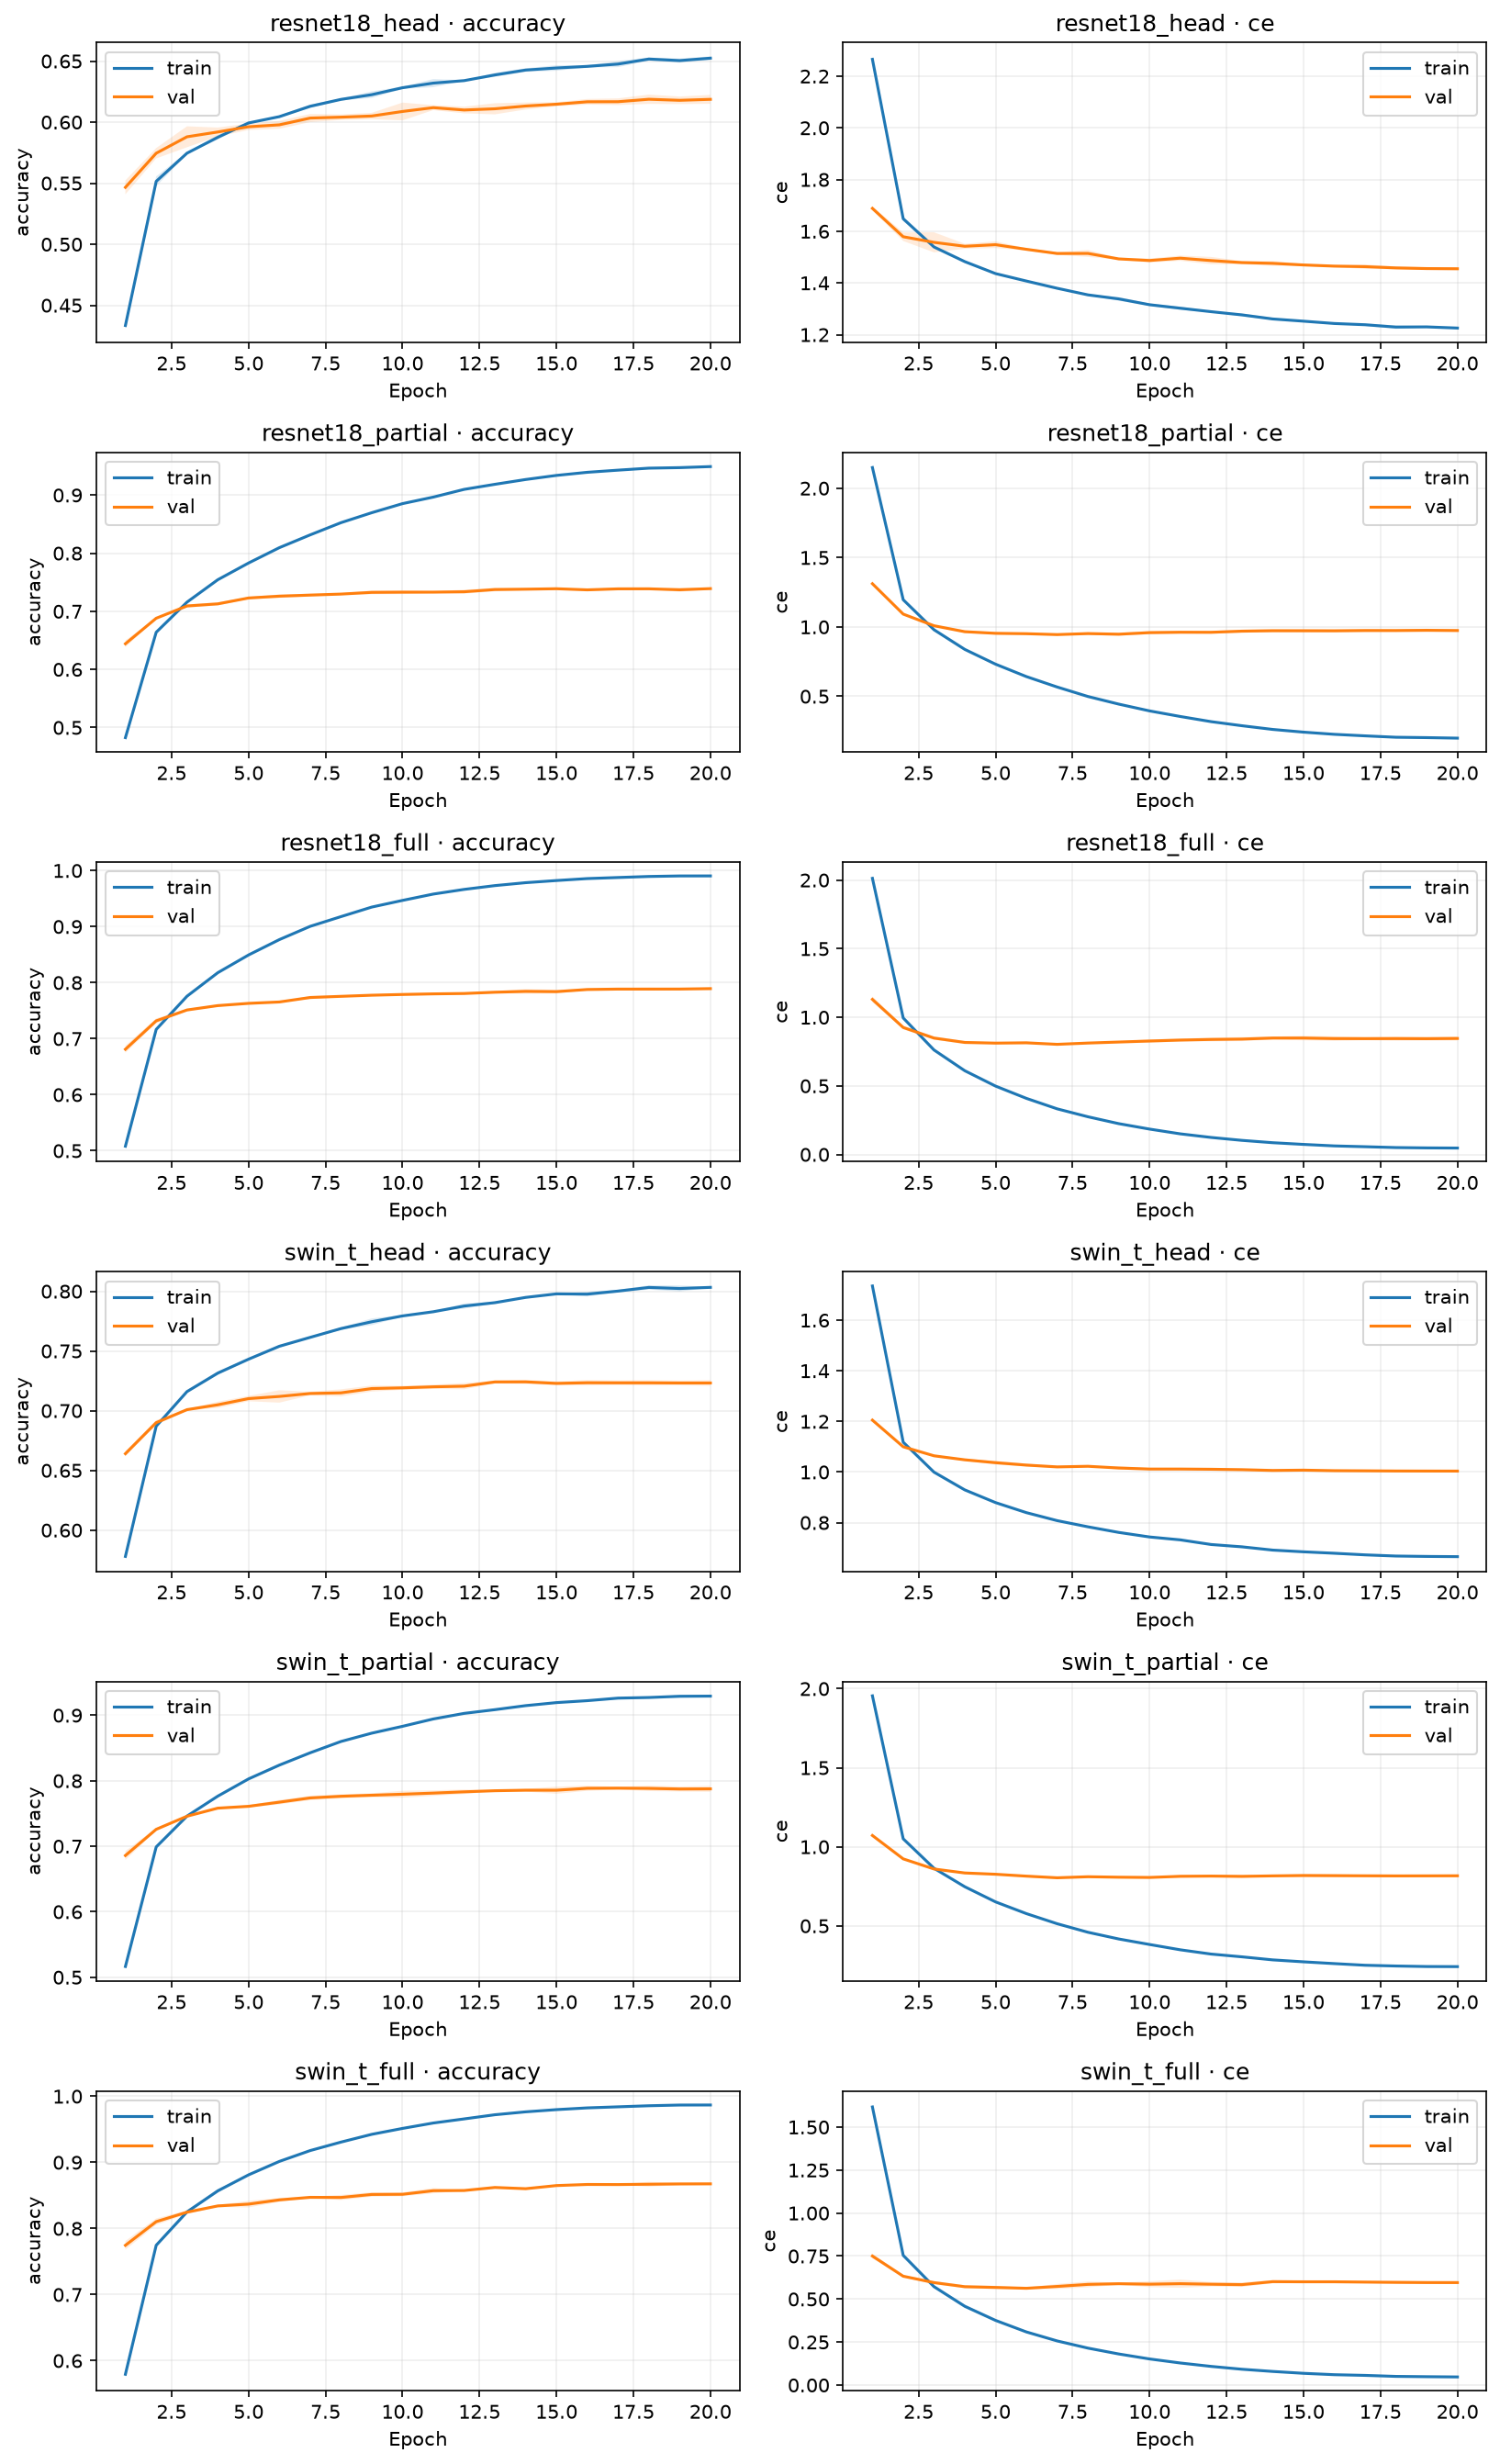
\includegraphics[trim=0 644pt 0 0,clip,width=\textwidth]{notebook-evidence/figures/learning_curves.png}
\caption{Accuracy và cross-entropy trên train/validation của ba cấu hình ResNet18 qua 20 epoch; đường cong tổng hợp từ các seed 42, 43 và 44.}
\end{figure}

\begin{figure}[htbp]\centering
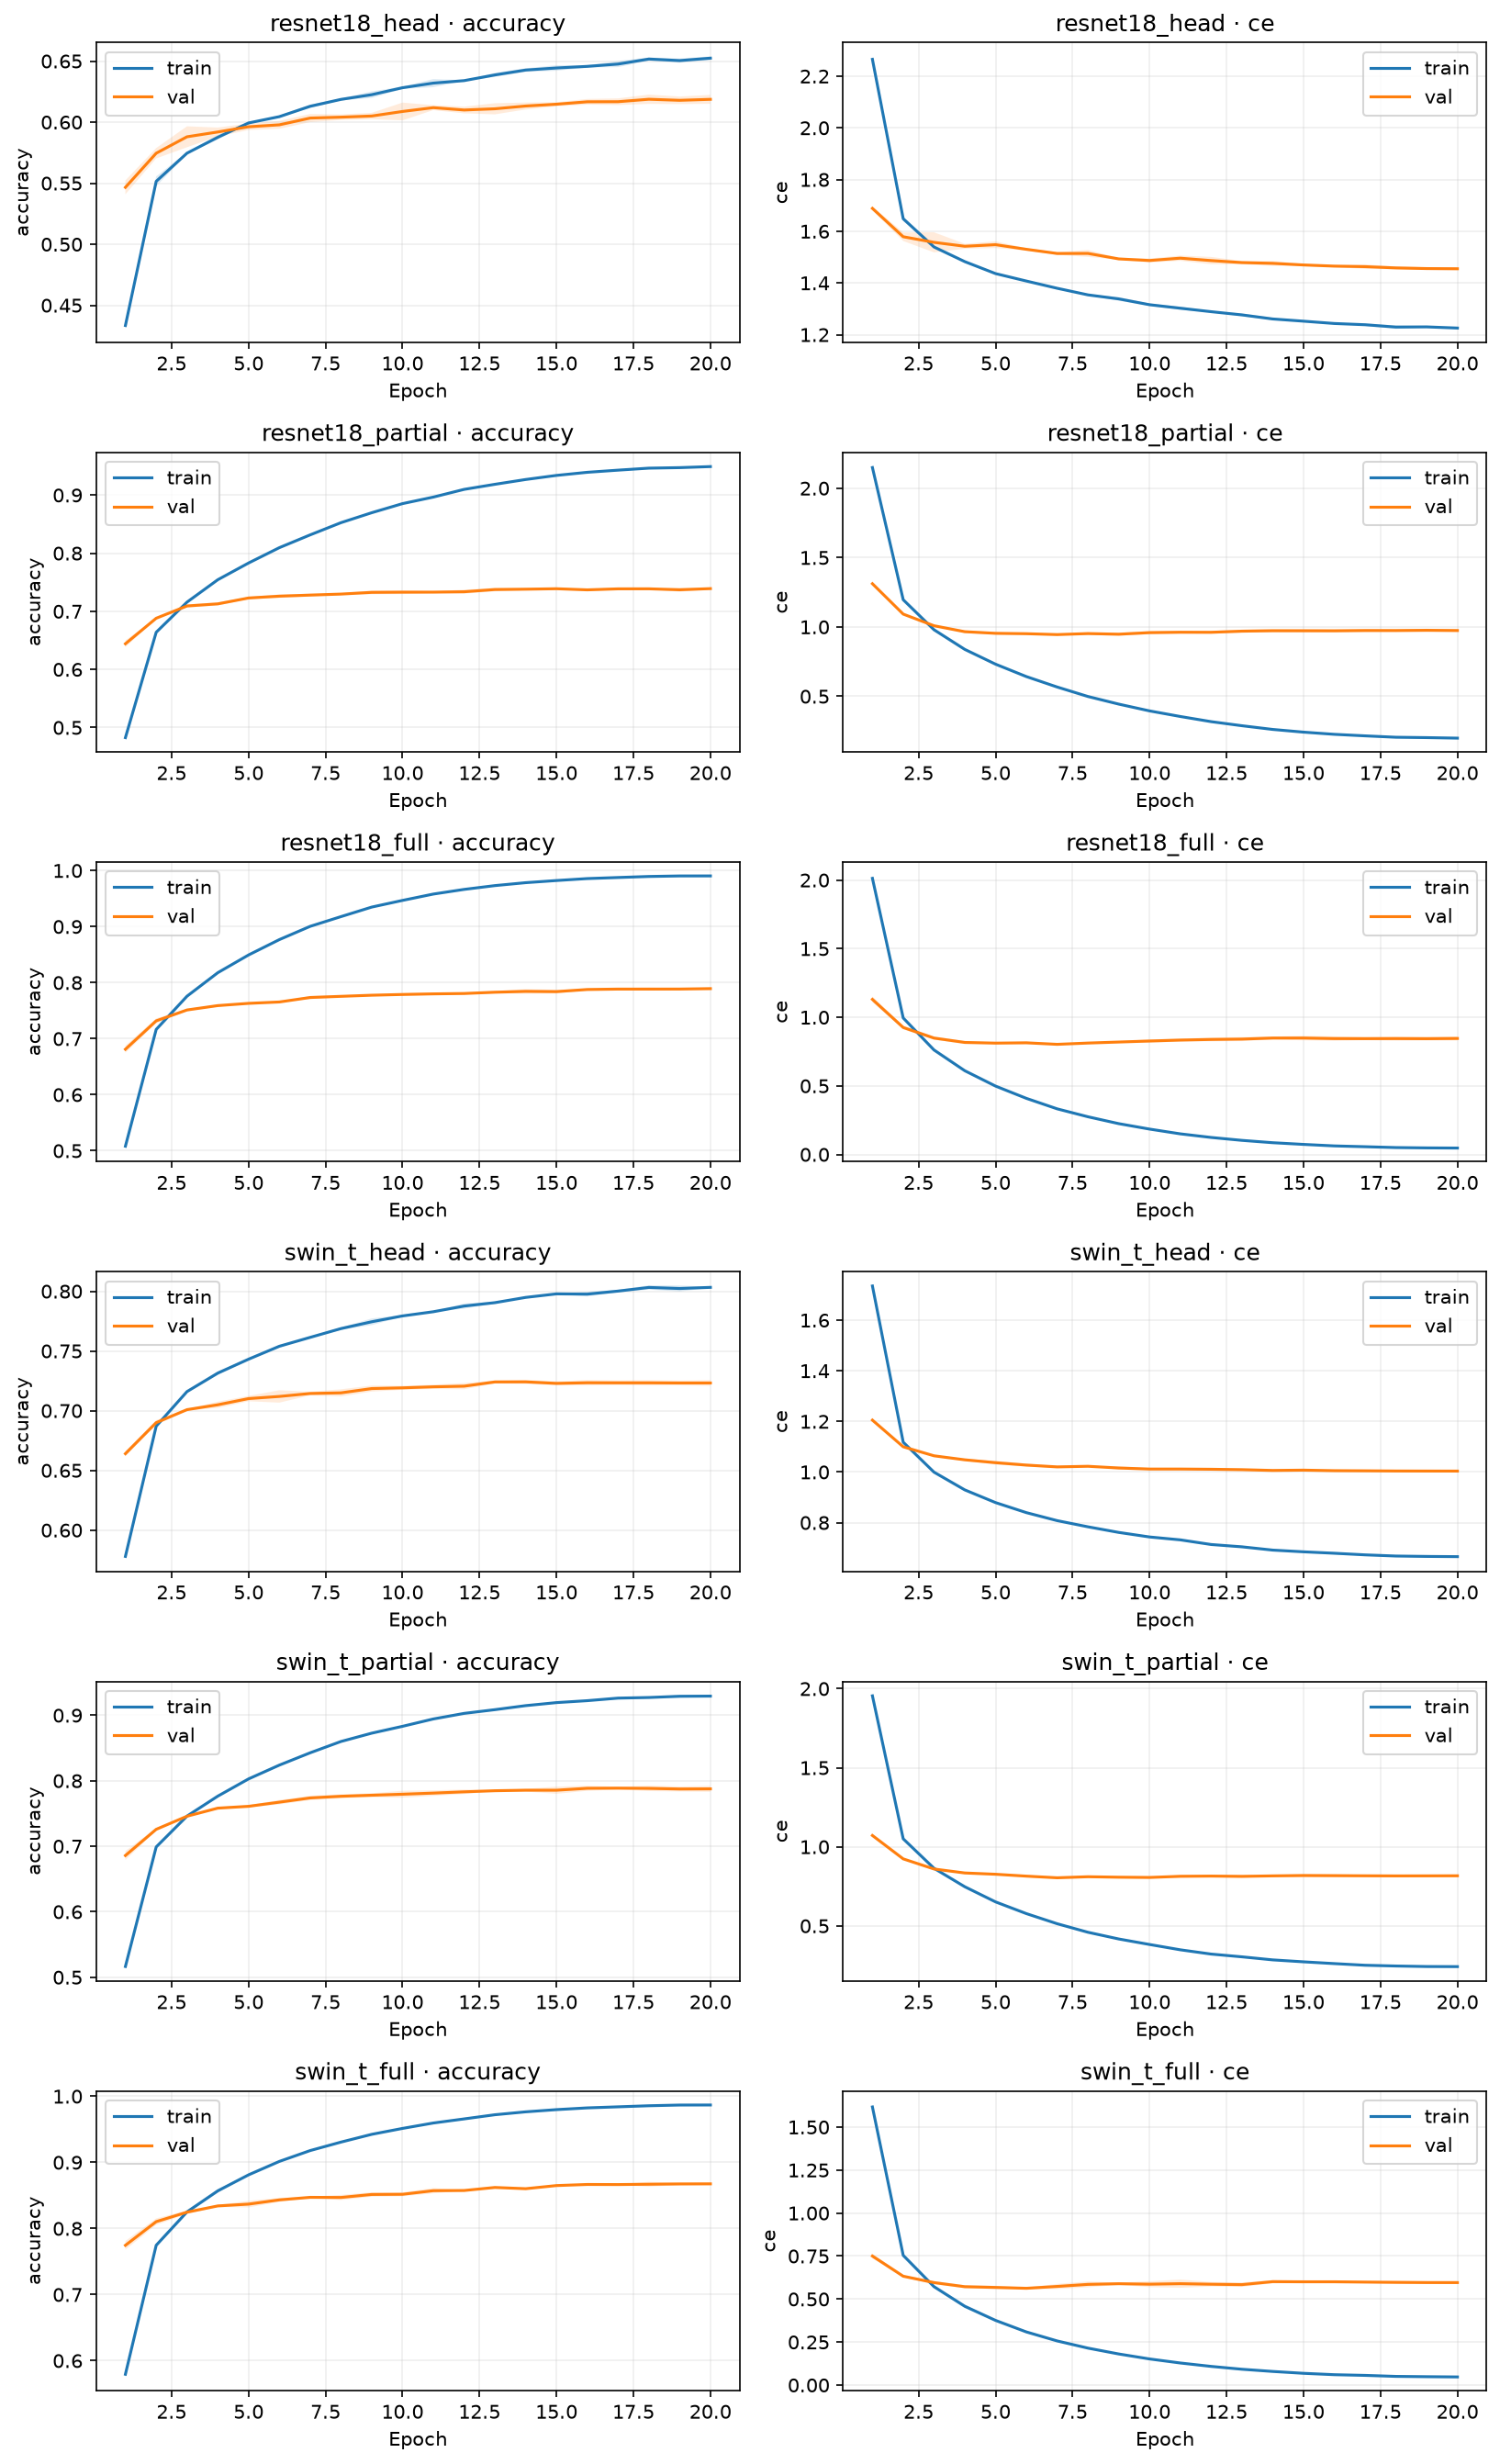
\includegraphics[trim=0 0 0 644pt,clip,width=\textwidth]{notebook-evidence/figures/learning_curves.png}
\caption{Accuracy và cross-entropy trên train/validation của ba cấu hình Swin-T qua 20 epoch; đường cong tổng hợp từ các seed 42, 43 và 44.}
\end{figure}

Các đường cong cho thấy accuracy trên tập train tiếp tục tăng trong khi mức cải thiện trên validation chậm lại. Ở epoch cuối, ResNet18 full đạt khoảng 99\% accuracy trên tập train nhưng chỉ khoảng 79\% trên validation; Swin-T full tương ứng khoảng 99\% và 87\%. Khoảng cách này cho thấy việc khớp tốt hơn với tập train không chuyển hoàn toàn thành chất lượng trên ảnh chưa dùng để cập nhật tham số. Do augmentation chỉ áp dụng trong train và số đo train được tích lũy khi tham số đang thay đổi, đây không phải phép so sánh hai tập trong điều kiện suy luận giống hệt nhau. Checkpoint vì vậy được chọn theo validation thay vì mặc định lấy epoch cuối.

\section{Chi phí và so sánh ghép cặp}

Swin-T full cao hơn ResNet18 full $7{,}66\pm0{,}41$ điểm phần trăm theo chênh lệch ghép cặp cùng seed; độ lệch chuẩn được tính từ ba chênh lệch theo seed. Macro-F1 của hai cấu hình lần lượt là $0{,}8681\pm0{,}0001$ và $0{,}7915\pm0{,}0038$.

\begin{table}[htbp]\centering\small
\begin{tabular}{lrr}
\toprule
Cấu hình & Thời gian train (s) & Peak allocated memory (MiB)\\\midrule
ResNet18 head-only & $79,0\pm0,2$ & $251,6\pm0,4$\\
ResNet18 partial & $79,5\pm0,1$ & $347,4\pm0,0$\\
ResNet18 full & $79,6\pm0,2$ & $520,4\pm0,0$\\
Swin-T head-only & $83,7\pm0,4$ & $501,9\pm0,0$\\
Swin-T partial & $104,8\pm0,1$ & $662,9\pm0,0$\\
Swin-T full & $209,6\pm0,1$ & $2454,2\pm0,0$\\
\bottomrule
\end{tabular}
\caption{Trên cùng RTX 5090 và bốn workers, Swin-T full đạt accuracy 86,81\% so với 79,16\% của ResNet18 full: mức tăng 7,66 điểm phần trăm theo ba cặp seed đi kèm 2,63 lần thời gian train và 4,72 lần bộ nhớ cấp phát cực đại. Chi phí là trung bình $\pm$ SD mẫu qua seed 42, 43 và 44; SD bộ nhớ làm tròn về 0,0 MiB ở năm cấu hình, riêng ResNet18 head-only là 0,4 MiB.}
\label{tab:new-image-cost}
\end{table}

Trong chế độ full, Swin-T mất thời gian gấp 2,63 lần và dùng peak memory gấp 4,72 lần ResNet18. Chỉ học head giảm bộ nhớ cấp phát cực đại ở cả hai backbone. Với Swin-T, thời gian train giảm từ 209,6 xuống 83,7 giây; với ResNet18, chênh lệch thời gian giữa ba mức fine-tuning chỉ khoảng 0,6 giây. Do thời gian đo bao gồm nạp dữ liệu và augmentation, không thể suy trực tiếp mức giảm phép tính backward từ mức giảm tổng thời gian này. Swin-T partial có accuracy gần ResNet18 full nhưng dùng nhiều thời gian và bộ nhớ hơn trong phép đo này; lợi thế accuracy rõ hơn của Swin-T xuất hiện ở full. Các tỷ lệ chi phí chỉ áp dụng cho cùng RTX 5090 và giao thức 20 epoch, chưa cho biết tốc độ suy luận hoặc hiệu quả trên phần cứng khác.

\section{Phân tích nhầm lẫn}

\begin{figure}[htbp]\centering
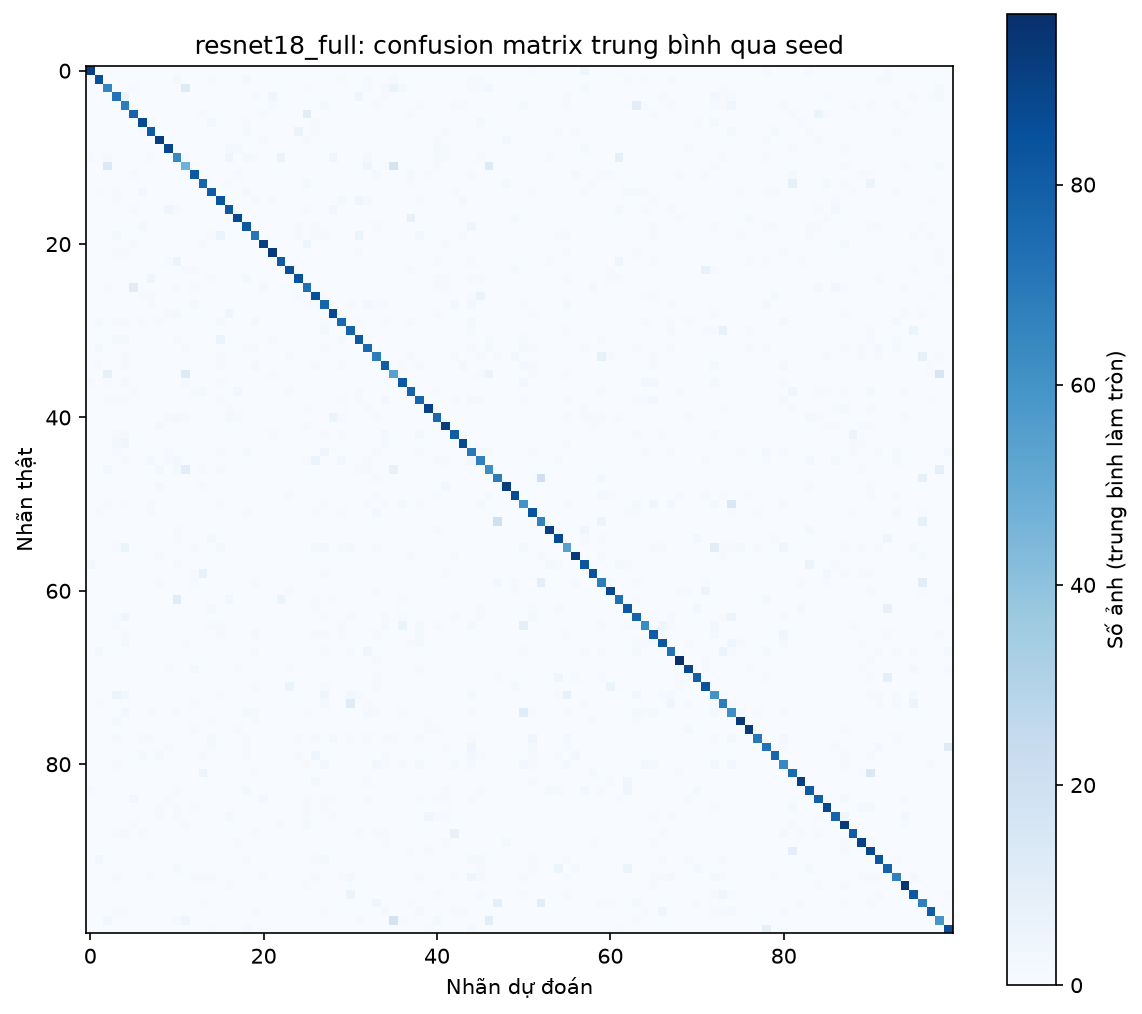
\includegraphics[width=.48\textwidth]{notebook-evidence/figures/resnet18_full-confusion.png}\hfill
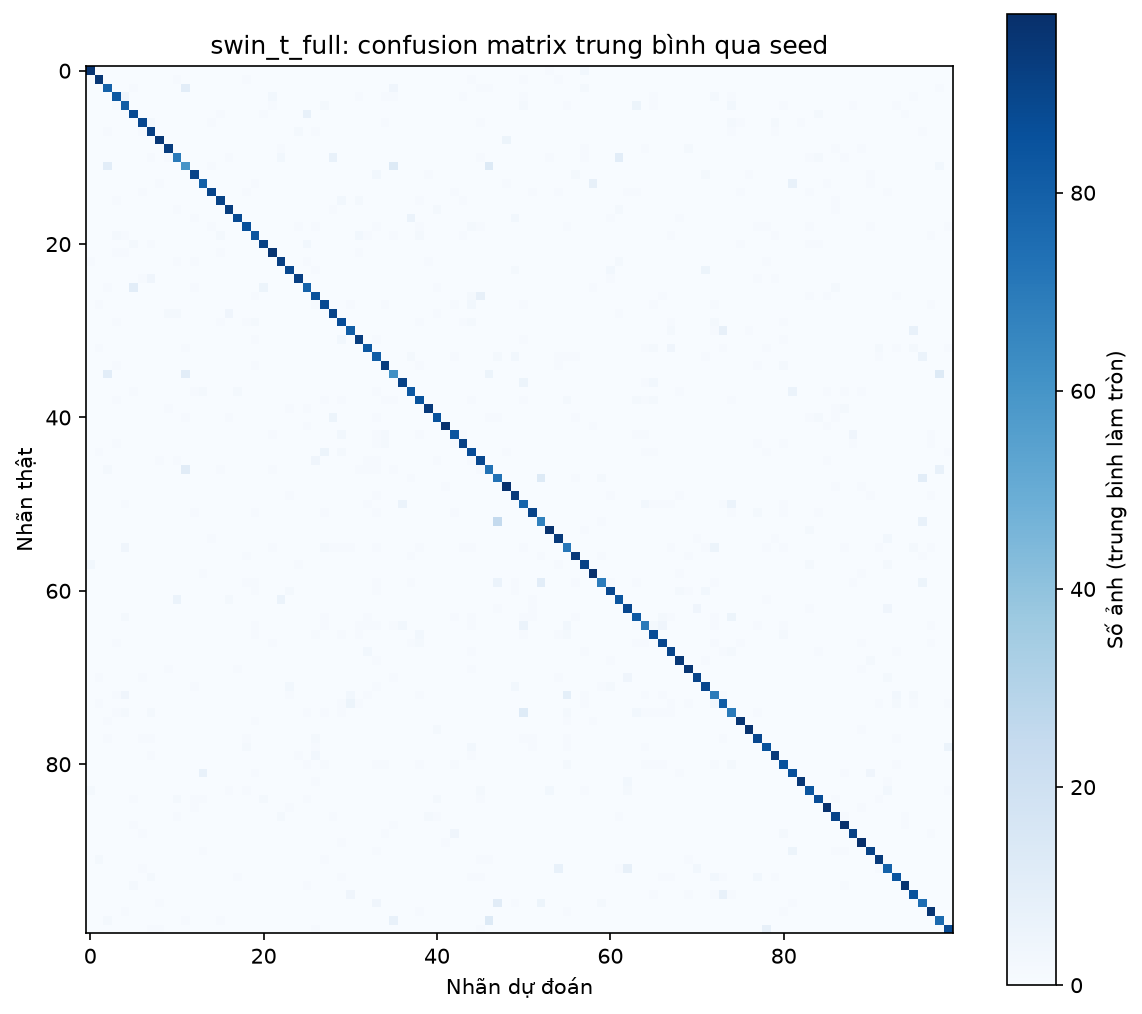
\includegraphics[width=.48\textwidth]{notebook-evidence/figures/swin_t_full-confusion.png}
\caption{Confusion matrix test trung bình qua các seed 42, 43 và 44: ResNet18 full (trái), Swin-T full (phải). Màu biểu diễn số ảnh trung bình tại mỗi ô; trục dùng chỉ số lớp từ 0 đến 99, không ghi số ảnh trong từng ô.}
\end{figure}

Trong confusion matrix, hàng biểu diễn nhãn đúng và cột biểu diễn nhãn dự đoán. Đường chéo ghi nhận dự đoán đúng, còn các ô ngoài đường chéo cho biết hướng nhầm lẫn cụ thể. Do hình gồm 100 lớp và không có nhãn tên lớp, Bảng~\ref{tab:image-confusion-pairs} bổ sung bốn hướng nhầm lẫn cùng chỉ số hàng, cột tương ứng.

\begin{table}[htbp]\centering\small
\begin{tabularx}{\textwidth}{@{}XXrr@{}}
\toprule
Nhãn đúng (hàng) & Nhãn dự đoán (cột) & ResNet18 full & Swin-T full\\\midrule
oak\_tree (52) & maple\_tree (47) & 19,00 & 23,67\\
maple\_tree (47) & oak\_tree (52) & 18,33 & 16,00\\
woman (98) & girl (35) & 16,67 & 9,67\\
girl (35) & woman (98) & 15,33 & 11,33\\
\bottomrule
\end{tabularx}
\caption{Số ảnh bị phân loại sai trung bình qua seed 42, 43 và 44 tại bốn ô ngoài đường chéo, làm tròn đến hai chữ số thập phân. Mỗi hàng là một hướng nhầm lẫn, không phải tổng hai chiều; chỉ số lớp bắt đầu từ 0 như trên hình.}
\label{tab:image-confusion-pairs}
\end{table}

Nhầm lẫn oak\_tree với maple\_tree vẫn nổi bật ở cả hai mô hình. Dù accuracy tổng thể cao hơn, Swin-T full có nhiều lỗi theo hướng oak\_tree sang maple\_tree hơn ResNet18 full, trong khi số lỗi ở chiều ngược lại thấp hơn. Với hai hướng woman--girl, số lỗi đều giảm ở Swin-T full. Như vậy, cải thiện accuracy tổng thể không đồng nghĩa với cải thiện ở mọi cặp lớp. Để giải thích các khác biệt này cần xem ảnh bị phân loại sai và so sánh đặc trưng; riêng confusion matrix chưa xác định được vai trò của độ phân giải, hình dạng vật thể hay kiến trúc.


\section{Kết luận}
Trong sáu cấu hình pretrained được đo, fine-tuning sâu hơn cải thiện accuracy ở cả ResNet18 và Swin-T. Swin-T full đạt accuracy và macro-F1 cao nhất, đồng thời tốn thêm thời gian và bộ nhớ so với ResNet18 full. Partial giảm bộ nhớ so với full nhưng cũng làm giảm accuracy; lựa chọn giữa hai chế độ phụ thuộc vào ngân sách tính toán và mức chất lượng cần đạt. Nhầm lẫn giữa oak\_tree và maple\_tree vẫn xuất hiện ở cả hai mô hình full. Kết luận áp dụng cho CIFAR-100, đầu vào 96 px, giao thức 20 epoch và phần cứng được mô tả ở trên.

\section{Giới hạn}
Cạnh ảnh gốc chỉ có 32 px, thấp hơn mức 128 px được khuyến nghị; resize lên 96 px không khôi phục chi tiết đã mất. Phân tích ảnh trùng chỉ phát hiện trùng pixel chính xác, chưa xét ảnh gần trùng. Thực nghiệm giới hạn ở một tập dữ liệu, hai kiến trúc, ba mức fine-tuning, ba seed và một GPU; không khảo sát train from scratch làm baseline hoặc thời lượng dài hơn. Cùng số epoch không đồng nghĩa với cùng chi phí tính toán, và chưa có tìm kiếm siêu tham số riêng cho từng kiến trúc. Ba seed chỉ phản ánh biến động do khởi tạo và quá trình train trên một cách chia dữ liệu cố định; SD nhỏ không phải khoảng tin cậy cho mọi cách chia dữ liệu hay mọi ảnh ngoài CIFAR-100.

Thông tin sử dụng AI được trình bày trong \href{https://github.com/dathuynh1108/CO5177-PFDAV/blob/main/AI_USE_REPORT.md}{AI\_USE\_REPORT.md}.

\begin{thebibliography}{9}
\addcontentsline{toc}{chapter}{Tài liệu tham khảo}
\bibitem{assignment} Lê Thành Sách. \emph{Course Assignment: Nền tảng lập trình cho phân tích và trực quan dữ liệu}. CO5177, v4.0, 14/09/2026.
\bibitem{cifar} A. Krizhevsky. \emph{Learning Multiple Layers of Features from Tiny Images}. 2009. \url{https://www.cs.toronto.edu/~kriz/cifar.html}.
\bibitem{resnet} K. He và cộng sự. \emph{Deep Residual Learning for Image Recognition}. CVPR 2016. \url{https://arxiv.org/abs/1512.03385}.
\bibitem{swin} Z. Liu và cộng sự. \emph{Swin Transformer: Hierarchical Vision Transformer using Shifted Windows}. ICCV 2021. \url{https://arxiv.org/abs/2103.14030}.
\bibitem{torchvision} Torchvision. ResNet18 và Swin-T model API; trọng số IMAGENET1K\_V1. \url{https://docs.pytorch.org/vision/stable/models.html}.
\end{thebibliography}
\end{document}
